\documentclass[
  shownotes,
  xcolor={svgnames},
  hyperref={colorlinks,citecolor=DarkBlue,linkcolor=DarkRed,urlcolor=DarkBlue}
  ]{beamer}
\usepackage{animate}
\usepackage{amsmath}
\usepackage{amsfonts}
\usepackage{amssymb}
\usepackage{pifont}
\usepackage{mathpazo}
%\usepackage{xcolor}
\usepackage{multimedia}
\usepackage{fancybox}
\usepackage[para]{threeparttable}
\usepackage{multirow}
\setcounter{MaxMatrixCols}{30}
\usepackage{subcaption}
\usepackage{graphicx}
\usepackage{lscape}
\usepackage[compatibility=false,font=small]{caption}
\usepackage{booktabs}
\usepackage{ragged2e}
\usepackage{chronosys}
\usepackage{appendixnumberbeamer}
\usepackage{animate}
\setbeamertemplate{caption}[numbered]
\usepackage{color}
%\usepackage{times}
\usepackage{tikz}
\usepackage{comment} %to comment
%% BibTeX settings
\usepackage{natbib}
\bibliographystyle{apalike}
\bibpunct{(}{)}{,}{a}{,}{,}
\setbeamertemplate{bibliography item}{[\theenumiv]}

% Defines columns for bespoke tables
\usepackage{array}
\newcolumntype{L}[1]{>{\raggedright\let\newline\\\arraybackslash\hspace{0pt}}m{#1}}
\newcolumntype{C}[1]{>{\centering\let\newline\\\arraybackslash\hspace{0pt}}m{#1}}
\newcolumntype{R}[1]{>{\raggedleft\let\newline\\\arraybackslash\hspace{0pt}}m{#1}}


\usepackage{xfrac}


\usepackage{multicol}
\setlength{\columnsep}{0.5cm}

% Theme and colors
\usetheme{Boadilla}

% I use steel blue and a custom color palette. This defines it.
\definecolor{andesred}{HTML}{af2433}

% Other options
\providecommand{\U}[1]{\protect\rule{.1in}{.1in}}
\usefonttheme{serif}
\setbeamertemplate{itemize items}[default]
\setbeamertemplate{enumerate items}[square]
\setbeamertemplate{section in toc}[circle]

\makeatletter

\definecolor{mybackground}{HTML}{82CAFA}
\definecolor{myforeground}{HTML}{0000A0}

\setbeamercolor{normal text}{fg=black,bg=white}
\setbeamercolor{alerted text}{fg=red}
\setbeamercolor{example text}{fg=black}

\setbeamercolor{background canvas}{fg=myforeground, bg=white}
\setbeamercolor{background}{fg=myforeground, bg=mybackground}

\setbeamercolor{palette primary}{fg=black, bg=gray!30!white}
\setbeamercolor{palette secondary}{fg=black, bg=gray!20!white}
\setbeamercolor{palette tertiary}{fg=white, bg=andesred}

\setbeamercolor{frametitle}{fg=andesred}
\setbeamercolor{title}{fg=andesred}
\setbeamercolor{block title}{fg=andesred}
\setbeamercolor{itemize item}{fg=andesred}
\setbeamercolor{itemize subitem}{fg=andesred}
\setbeamercolor{itemize subsubitem}{fg=andesred}
\setbeamercolor{enumerate item}{fg=andesred}
\setbeamercolor{item projected}{bg=gray!30!white,fg=andesred}
\setbeamercolor{enumerate subitem}{fg=andesred}
\setbeamercolor{section number projected}{bg=gray!30!white,fg=andesred}
\setbeamercolor{section in toc}{fg=andesred}
\setbeamercolor{caption name}{fg=andesred}
\setbeamercolor{button}{bg=gray!30!white,fg=andesred}


\usepackage{fancyvrb}
\newcommand{\VerbBar}{|}
\newcommand{\VERB}{\Verb[commandchars=\\\{\}]}
\DefineVerbatimEnvironment{Highlighting}{Verbatim}{commandchars=\\\{\}}
% Add ',fontsize=\small' for more characters per line
\usepackage{framed}
\definecolor{shadecolor}{RGB}{248,248,248}
\newenvironment{Shaded}{\begin{snugshade}}{\end{snugshade}}
\newcommand{\AlertTok}[1]{\textcolor[rgb]{0.94,0.16,0.16}{#1}}
\newcommand{\AnnotationTok}[1]{\textcolor[rgb]{0.56,0.35,0.01}{\textbf{\textit{#1}}}}
\newcommand{\AttributeTok}[1]{\textcolor[rgb]{0.77,0.63,0.00}{#1}}
\newcommand{\BaseNTok}[1]{\textcolor[rgb]{0.00,0.00,0.81}{#1}}
\newcommand{\BuiltInTok}[1]{#1}
\newcommand{\CharTok}[1]{\textcolor[rgb]{0.31,0.60,0.02}{#1}}
\newcommand{\CommentTok}[1]{\textcolor[rgb]{0.56,0.35,0.01}{\textit{#1}}}
\newcommand{\CommentVarTok}[1]{\textcolor[rgb]{0.56,0.35,0.01}{\textbf{\textit{#1}}}}
\newcommand{\ConstantTok}[1]{\textcolor[rgb]{0.00,0.00,0.00}{#1}}
\newcommand{\ControlFlowTok}[1]{\textcolor[rgb]{0.13,0.29,0.53}{\textbf{#1}}}
\newcommand{\DataTypeTok}[1]{\textcolor[rgb]{0.13,0.29,0.53}{#1}}
\newcommand{\DecValTok}[1]{\textcolor[rgb]{0.00,0.00,0.81}{#1}}
\newcommand{\DocumentationTok}[1]{\textcolor[rgb]{0.56,0.35,0.01}{\textbf{\textit{#1}}}}
\newcommand{\ErrorTok}[1]{\textcolor[rgb]{0.64,0.00,0.00}{\textbf{#1}}}
\newcommand{\ExtensionTok}[1]{#1}
\newcommand{\FloatTok}[1]{\textcolor[rgb]{0.00,0.00,0.81}{#1}}
\newcommand{\FunctionTok}[1]{\textcolor[rgb]{0.00,0.00,0.00}{#1}}
\newcommand{\ImportTok}[1]{#1}
\newcommand{\InformationTok}[1]{\textcolor[rgb]{0.56,0.35,0.01}{\textbf{\textit{#1}}}}
\newcommand{\KeywordTok}[1]{\textcolor[rgb]{0.13,0.29,0.53}{\textbf{#1}}}
\newcommand{\NormalTok}[1]{#1}
\newcommand{\OperatorTok}[1]{\textcolor[rgb]{0.81,0.36,0.00}{\textbf{#1}}}
\newcommand{\OtherTok}[1]{\textcolor[rgb]{0.56,0.35,0.01}{#1}}
\newcommand{\PreprocessorTok}[1]{\textcolor[rgb]{0.56,0.35,0.01}{\textit{#1}}}
\newcommand{\RegionMarkerTok}[1]{#1}
\newcommand{\SpecialCharTok}[1]{\textcolor[rgb]{0.00,0.00,0.00}{#1}}
\newcommand{\SpecialStringTok}[1]{\textcolor[rgb]{0.31,0.60,0.02}{#1}}
\newcommand{\StringTok}[1]{\textcolor[rgb]{0.31,0.60,0.02}{#1}}
\newcommand{\VariableTok}[1]{\textcolor[rgb]{0.00,0.00,0.00}{#1}}
\newcommand{\VerbatimStringTok}[1]{\textcolor[rgb]{0.31,0.60,0.02}{#1}}
\newcommand{\WarningTok}[1]{\textcolor[rgb]{0.56,0.35,0.01}{\textbf{\textit{#1}}}}
\usepackage{graphicx}
\makeatletter

\definecolor{airforceblue}{rgb}{0.36, 0.54, 0.66}

\usepackage{tikz}
% Tikz settings optimized for causal graphs.
\usetikzlibrary{shapes,decorations,arrows,calc,arrows.meta,fit,positioning}
\tikzset{
    -Latex,auto,node distance =1 cm and 1 cm,semithick,
    state/.style ={ellipse, draw, minimum width = 0.7 cm},
    point/.style = {circle, draw, inner sep=0.04cm,fill,node contents={}},
    bidirected/.style={Latex-Latex,dashed},
    el/.style = {inner sep=2pt, align=left, sloped}
}


\makeatother






%%%%%%%%%%%%%%% BEGINS DOCUMENT %%%%%%%%%%%%%%%%%%

\begin{document}

\title[Lecture 16]{Lecture 16: \\ Regularization/Shrinkage Methods}
\subtitle{Big Data and Machine Learning for Applied Economics \\ Econ 4676}
\date{\today}

\author[Sarmiento-Barbieri]{Ignacio Sarmiento-Barbieri}
\institute[Uniandes]{Universidad de los Andes}


\begin{frame}[noframenumbering]
\maketitle
\end{frame}

%%%%%%%%%%%%%%%%%%%%%%%%%%%%%%%%%%%



%----------------------------------------------------------------------% 

\begin{frame}
\frametitle{Agenda}

\tableofcontents

\end{frame}

%----------------------------------------------------------------------%
\section{Recap \& Implementation}
\subsection{K-Fold Cross Validation}
%----------------------------------------------------------------------%
\begin{frame}[fragile]
\frametitle{Overfit and out of Sample Prediction}


\begin{itemize}
  \item ML we care about prediction out of sample
  \medskip
  \item Overfit: complex models predict very well inside a sample but "bad" outside
  \medskip
  \item Choose the right complexity level
  \medskip
  \item Trade off Bias/Variance
  \medskip
  \item Challenge: accept some bias to decrease variance
\end{itemize}

\end{frame}

%----------------------------------------------------------------------%
\begin{frame}[fragile]
\frametitle{Motivation}
\begin{itemize}
\item Estimating test error: two approaches
\medskip
\begin{enumerate}
\item We can directly estimate the test error, using either a validation set approach or a cross-validation approach
\medskip
\item We can indirectly estimate test error by making an adjustment to the training error to account for overfitting.
\medskip
\begin{itemize}
  \item AIC, BIC, $C_p$ and Adjusted $R^2$
  \medskip
  \item These techniques adjust the training error for the model size, and can be used to select among a set of models with different numbers of variables.
  \medskip
  \item AIC and BIC are very closely related to classical notions of hypothesis testing. 
\end{itemize}


\end{enumerate}
\end{itemize}

\end{frame}
%----------------------------------------------------------------------%
\begin{frame}[fragile]
\frametitle{Demo: Prelogomenon}

\begin{scriptsize}
\begin{Shaded}
\begin{Highlighting}[]
\CommentTok{\#Load the required packages}
\KeywordTok{library}\NormalTok{(}\StringTok{"McSpatial"}\NormalTok{) }\CommentTok{\#loads the package}
\KeywordTok{library}\NormalTok{(}\StringTok{"dplyr"}\NormalTok{) }\CommentTok{\#for data wrangling}
\KeywordTok{library}\NormalTok{(}\StringTok{"caret"}\NormalTok{) }\CommentTok{\#ML}
\KeywordTok{data}\NormalTok{(matchdata) }\CommentTok{\#loads the data set}
\NormalTok{matchdata \textless{}{-}}\StringTok{ }\NormalTok{matchdata }\OperatorTok{\%\textgreater{}\%}\StringTok{ }\KeywordTok{mutate}\NormalTok{(}\DataTypeTok{price=}\KeywordTok{exp}\NormalTok{(lnprice)) }\OperatorTok{\%\textgreater{}\%}\StringTok{ }\KeywordTok{select}\NormalTok{(}\OperatorTok{{-}}\NormalTok{lnprice) }
\CommentTok{\#transforms log prices to standard prices}
\KeywordTok{set.seed}\NormalTok{(}\DecValTok{123}\NormalTok{) }\CommentTok{\#set the seed for replication purposes}
\KeywordTok{str}\NormalTok{(matchdata) }\CommentTok{\#compact display}
\end{Highlighting}
\end{Shaded}
\end{scriptsize}
\begin{tiny}
\begin{verbatim}
## 'data.frame':    3204 obs. of  18 variables:
##  $ year     : num  1995 1995 1995 2005 1995 ...
##  $ lnland   : num  8.23 8.63 8.7 8.63 8.63 ...
##  $ lnbldg   : num  6.98 7.02 7.22 6.87 7.2 ...
##  $ rooms    : int  5 5 5 4 6 7 7 6 4 6 ...
##  $ bedrooms : int  3 3 3 2 3 3 4 3 2 3 ...
##  $ bathrooms: num  1 1.5 1.5 1 1 2 1 2 1.5 1.5 ...
##  $ centair  : int  0 1 1 0 1 0 1 1 1 1 ...
##  $ fireplace: int  0 0 0 0 0 1 0 0 0 0 ...
##  $ brick    : num  1 1 1 1 1 1 1 1 1 1 ...
##  $ garage1  : num  1 0 0 1 0 1 0 0 1 0 ...
##  $ garage2  : num  0 1 1 0 1 0 1 0 0 0 ...
##  $ dcbd     : num  13.6 13.5 13.6 13.5 13.6 ...
##  $ rr       : num  0 0 0 0 0 0 0 0 0 0 ...
##  $ yrbuilt  : num  1953 1952 1952 1949 1953 ...
##  $ carea    : Factor w/ 11 levels "Albany Park",..: 3 3 3 3 3 3 3 3 3 3 ...
##  $ latitude : num  42 42 42 42 42 ...
##  $ longitude: num  -87.8 -87.8 -87.8 -87.8 -87.8 ...
##  $ price    : num  170750 168000 192500 398000 215000 ...
\end{verbatim}
\end{tiny}

\end{frame}


%----------------------------------------------------------------------%
\begin{frame}[fragile]
\frametitle{Demo: K-fold CV}

\begin{scriptsize}
\begin{Shaded}
\begin{Highlighting}[]
\NormalTok{model2 \textless{}{-}}\StringTok{ }\KeywordTok{train}\NormalTok{(price }\OperatorTok{\textasciitilde{}}\StringTok{ }\NormalTok{bedrooms,   }\CommentTok{\# model to fit}
                     \DataTypeTok{data =}\NormalTok{ matchdata,                        }
                     \DataTypeTok{trControl =} \KeywordTok{trainControl}\NormalTok{(}\DataTypeTok{method =} \StringTok{"cv"}\NormalTok{, }\DataTypeTok{number =} \DecValTok{10}\NormalTok{),     }
                     \CommentTok{\# Method: crossvalidation, 10 folds}
                     \DataTypeTok{method =} \StringTok{"lm"}\NormalTok{)}\CommentTok{\# specifying regression model}

\NormalTok{model2}
\end{Highlighting}
\end{Shaded}
\end{scriptsize}
\begin{tiny}
\begin{verbatim}
## Linear Regression 
## 
## 3204 samples
##    1 predictor
## 
## No pre-processing
## Resampling: Cross-Validated (10 fold) 
## Summary of sample sizes: 2883, 2884, 2884, 2883, 2884, 2885, ... 
## Resampling results:
## 
##   RMSE      Rsquared    MAE     
##   147308.8  0.01385314  122117.8
## 
## Tuning parameter 'intercept' was held constant at a value of TRUE
\end{verbatim}
\end{tiny}
\end{frame}

%----------------------------------------------------------------------%
\begin{frame}[fragile]
\frametitle{Demo: K-fold CV}

\begin{scriptsize}
\begin{Shaded}
\begin{Highlighting}[]
\NormalTok{model2 \textless{}{-}}\StringTok{ }\KeywordTok{train}\NormalTok{(price }\OperatorTok{\textasciitilde{}}\StringTok{ }\NormalTok{bedrooms}\OperatorTok{+}\NormalTok{bathrooms}\OperatorTok{+}\StringTok{ }\NormalTok{rooms}\OperatorTok{+}\NormalTok{centair}\OperatorTok{+}\NormalTok{fireplace}\OperatorTok{+}\NormalTok{brick}\OperatorTok{+}
\StringTok{                        }\NormalTok{lnland}\OperatorTok{+}\NormalTok{lnbldg}\OperatorTok{+}\NormalTok{garage1}\OperatorTok{+}\NormalTok{garage2}\OperatorTok{+}
\StringTok{                        }\NormalTok{dcbd}\OperatorTok{+}\StringTok{ }\NormalTok{rr }\OperatorTok{+}
\StringTok{                        }\NormalTok{yrbuilt}\OperatorTok{+}\StringTok{ }\KeywordTok{factor}\NormalTok{(year) }\OperatorTok{+}
\StringTok{                        }\NormalTok{carea}\OperatorTok{+}\StringTok{ }\NormalTok{latitude}\OperatorTok{+}\NormalTok{longitude,}
                        \DataTypeTok{data =}\NormalTok{ matchdata,                        }
                        \DataTypeTok{trControl =} \KeywordTok{trainControl}\NormalTok{(}\DataTypeTok{method =} \StringTok{"cv"}\NormalTok{, }\DataTypeTok{number =} \DecValTok{10}\NormalTok{), }
                        \DataTypeTok{method =} \StringTok{"lm"}\NormalTok{)}
 
\NormalTok{model2}
\end{Highlighting}
\end{Shaded}
\end{scriptsize}
\begin{tiny}
\begin{verbatim}
## Linear Regression 
## 
## 3204 samples
##   17 predictor
## 
## No pre-processing
## Resampling: Cross-Validated (10 fold) 
## Summary of sample sizes: 2883, 2884, 2884, 2883, 2883, 2884, ... 
## Resampling results:
## 
##   RMSE      Rsquared   MAE     
##   74297.54  0.7490674  48170.37
## 
## Tuning parameter 'intercept' was held constant at a value of TRUE
\end{verbatim}
\end{tiny}

\end{frame}

%----------------------------------------------------------------------%
\frametitle{Model Subset Selection}
%----------------------------------------------------------------------%
\begin{frame}[fragile]
\frametitle{Model Subset Selection}

\begin{itemize}
\item We have $M_k$ models 
\bigskip
\item We want to find the model that best predicts out of sample
\bigskip
\item We have a number of ways to go about it
\bigskip
\begin{itemize}
  \item Best Subset Selection
  \medskip
  \item Stepwise Selection
  \begin{itemize}
    \item Forward selection
    \medskip
    \item Backward selection
  \end{itemize}
\end{itemize}
\end{itemize}
\end{frame}


%----------------------------------------------------------------------%
\begin{frame}[fragile]
\frametitle{Best Subset Selection}
\begin{align}
  y = \beta_0 + \beta_1 X_1 + \dots + \beta_p X_p +u
\end{align}

\begin{enumerate}
\item Estimate {\it \bf all} possible models with $k=0,1,..., p$ predictors.
\bigskip
\item Compute the prediction error using cross validation

\bigskip
\item  Pick the one with the smallest prediction error 
\end{enumerate}

\end{frame}





%----------------------------------------------------------------------%
\begin{frame}[fragile]
\frametitle{Demo: Best Subset Selection}
\begin{itemize}
 \item \texttt{Caret} is usually the solution but it doesn't have everything =(
\end{itemize}
 \begin{figure}[H] \centering
            \captionsetup{justification=centering}
              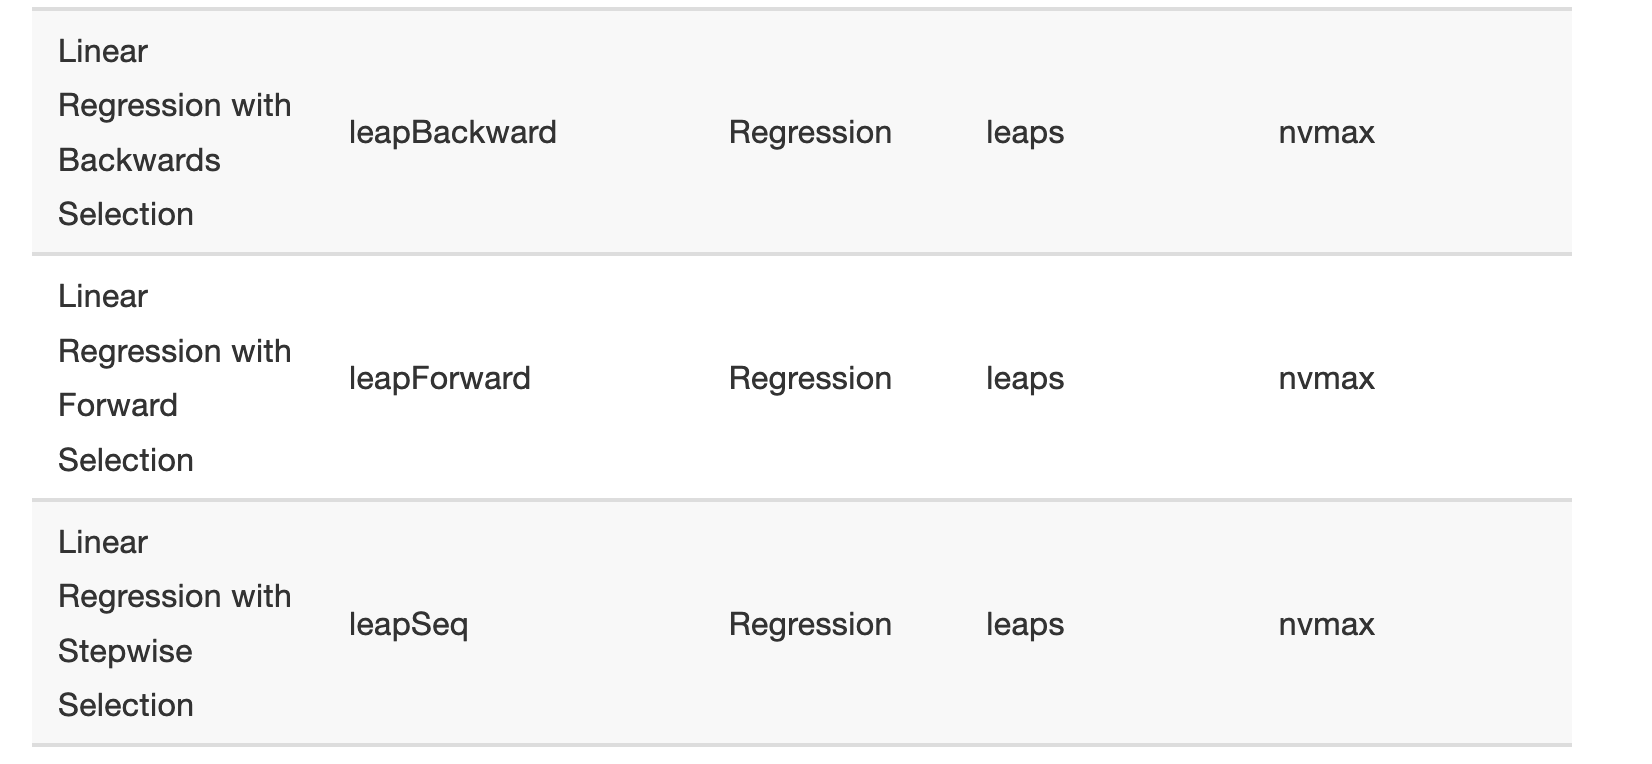
\includegraphics[scale=0.3]{figures/caret_leaps}
\\
\flushleft
              \scriptsize
              Note: \url{https://topepo.github.io/caret/available-models.html}
 \end{figure}


\end{frame}
%----------------------------------------------------------------------%
\begin{frame}[fragile]
\frametitle{Demo: Best Subset Selection}
\begin{Shaded}
\begin{Highlighting}[]
\KeywordTok{require}\NormalTok{(}\StringTok{"leaps"}\NormalTok{)}
\end{Highlighting}
\end{Shaded}

\begin{scriptsize}
\begin{Shaded}
\begin{Highlighting}[]
\KeywordTok{class}\NormalTok{(matchdata}\OperatorTok{$}\NormalTok{carea)}
\end{Highlighting}
\end{Shaded}

\begin{verbatim}
## [1] "factor"
\end{verbatim}

\begin{Shaded}
\begin{Highlighting}[]
\KeywordTok{class}\NormalTok{(matchdata}\OperatorTok{$}\NormalTok{year)}
\end{Highlighting}
\end{Shaded}

\begin{verbatim}
## [1] "numeric"
\end{verbatim}
\begin{Shaded}
\begin{Highlighting}[]
\NormalTok{matchdata}\OperatorTok{$}\NormalTok{year\textless{}{-}}\KeywordTok{factor}\NormalTok{(matchdata}\OperatorTok{$}\NormalTok{year)}
\end{Highlighting}
\end{Shaded}

\begin{Shaded}
\begin{Highlighting}[]
\NormalTok{best\textless{}{-}}\KeywordTok{regsubsets}\NormalTok{(price }\OperatorTok{\textasciitilde{}}\StringTok{ }\NormalTok{., }\DataTypeTok{method=}\StringTok{"exhaustive"}\NormalTok{,}\DataTypeTok{data =}\NormalTok{ matchdata)}
\KeywordTok{summary}\NormalTok{(best)}
\end{Highlighting}
\end{Shaded}
\end{scriptsize}

\end{frame}

%----------------------------------------------------------------------%
\begin{frame}[fragile]
\frametitle{Demo: Best Subset Selection}

\begin{tiny}
\begin{verbatim}
## Subset selection object
## Call: regsubsets.formula(price ~ ., method = "exhaustive", data = matchdata)
## 26 Variables  (and intercept)
## ...
## Selection Algorithm: exhaustive
##          year2005 lnland lnbldg rooms bedrooms bathrooms centair fireplace
## 1  ( 1 ) "*"      " "    " "    " "   " "      " "       " "     " "      
## 2  ( 1 ) "*"      " "    "*"    " "   " "      " "       " "     " "      
## 3  ( 1 ) "*"      "*"    "*"    " "   " "      " "       " "     " "      
## 4  ( 1 ) "*"      "*"    "*"    " "   " "      " "       " "     " "      
## 5  ( 1 ) "*"      "*"    "*"    " "   " "      " "       " "     " "      
## 6  ( 1 ) "*"      "*"    "*"    " "   " "      " "       " "     " "      
## 7  ( 1 ) "*"      "*"    "*"    " "   " "      " "       " "     " "      
## 8  ( 1 ) "*"      "*"    "*"    " "   " "      " "       " "     "*"      
##          brick garage1 garage2 dcbd rr  yrbuilt careaEdgewater careaEdison Park
## 1  ( 1 ) " "   " "     " "     " "  " " " "     " "            " "             
## 2  ( 1 ) " "   " "     " "     " "  " " " "     " "            " "             
## 3  ( 1 ) " "   " "     " "     " "  " " " "     " "            " "             
## 4  ( 1 ) " "   " "     " "     " "  " " " "     "*"            " "             
## 5  ( 1 ) " "   " "     " "     " "  " " " "     "*"            " "             
## 6  ( 1 ) " "   " "     " "     " "  " " " "     "*"            " "             
## 7  ( 1 ) " "   " "     " "     " "  " " " "     "*"            " "             
## 8  ( 1 ) " "   " "     " "     " "  " " " "     "*"            " "      
\end{verbatim}
\end{tiny}
\end{frame}
%----------------------------------------------------------------------%
\begin{frame}[fragile]
\frametitle{Demo: Best Subset Selection}
\begin{tiny}
\begin{verbatim}       
##          careaForest Glen careaJefferson Park careaLincoln Square
## 1  ( 1 ) " "              " "                 " "                
## 2  ( 1 ) " "              " "                 " "                
## 3  ( 1 ) " "              " "                 " "                
## 4  ( 1 ) " "              " "                 " "                
## 5  ( 1 ) "*"              " "                 " "                
## 6  ( 1 ) "*"              " "                 " "                
## 7  ( 1 ) "*"              " "                 "*"                
## 8  ( 1 ) "*"              " "                 "*"                
##          careaNorth Park careaNorwood Park careaRogers Park careaUptown
## 1  ( 1 ) " "             " "               " "              " "        
## 2  ( 1 ) " "             " "               " "              " "        
## 3  ( 1 ) " "             " "               " "              " "        
## 4  ( 1 ) " "             " "               " "              " "        
## 5  ( 1 ) " "             " "               " "              " "        
## 6  ( 1 ) " "             " "               " "              "*"        
## 7  ( 1 ) " "             " "               " "              "*"        
## 8  ( 1 ) " "             " "               " "              "*"        
##          careaWest Ridge latitude longitude
## 1  ( 1 ) " "             " "      " "      
## 2  ( 1 ) " "             " "      " "      
## 3  ( 1 ) " "             " "      " "      
## 4  ( 1 ) " "             " "      " "      
## 5  ( 1 ) " "             " "      " "      
## 6  ( 1 ) " "             " "      " "      
## 7  ( 1 ) " "             " "      " "      
## 8  ( 1 ) " "             " "      " "
\end{verbatim}
\end{tiny}
\end{frame}


%----------------------------------------------------------------------%
\begin{frame}[fragile]
\frametitle{Stepwise Selection}
 
 \begin{enumerate}
 \item Forward Stepwise Selection
 \begin{itemize}
\item Start with no predictors
\medskip
\item Test all models with 1 predictor. Choose the one with smallest prediction error using cross validation
\medskip
\item Add 1 predictor at a time, without taking away. 
\medskip
\item Of the p+1 models, choose the one with smallest prediction error using cross validation
\end{itemize}
\item  Backward Stepwise Selection
\begin{itemize}
  \item Same idea but start with a complete model and go backwards, taking one at a time. 
  \end{itemize}
\end{enumerate}
\end{frame}
%----------------------------------------------------------------------%
\begin{frame}[fragile]
\frametitle{Demo Stepwise Selection}

\begin{scriptsize}
\begin{Shaded}
\begin{Highlighting}[]
\NormalTok{forward \textless{}{-}}\StringTok{ }\KeywordTok{train}\NormalTok{(price }\OperatorTok{\textasciitilde{}}\StringTok{ }\NormalTok{., }\DataTypeTok{data =}\NormalTok{ matchdata,}
              \DataTypeTok{method =} \StringTok{"leapForward"}\NormalTok{,}
              \DataTypeTok{trControl =} \KeywordTok{trainControl}\NormalTok{(}\DataTypeTok{method =} \StringTok{"cv"}\NormalTok{, }\DataTypeTok{number =} \DecValTok{10}\NormalTok{))}
\NormalTok{forward}
\end{Highlighting}
\end{Shaded}
\end{scriptsize}
\begin{tiny}
\begin{verbatim}
## Linear Regression with Forward Selection 
## 
## 3204 samples
##   17 predictor
## 
## No pre-processing
## Resampling: Cross-Validated (10 fold) 
## Summary of sample sizes: 2884, 2884, 2884, 2883, 2883, 2883, ... 
## Resampling results across tuning parameters:
## 
##   nvmax  RMSE      Rsquared   MAE     
##   2      84219.28  0.6768962  55184.58
##   3      79212.49  0.7147519  51009.82
##   4      78595.00  0.7193113  50631.17
## 
## RMSE was used to select the optimal model using the smallest value.
## The final value used for the model was nvmax = 4.
\end{verbatim}
\end{tiny}


\end{frame}
%----------------------------------------------------------------------%
\begin{frame}[fragile]
\frametitle{Demo Stepwise Selection}

\begin{scriptsize}
\begin{Shaded}
\begin{Highlighting}[]
\KeywordTok{summary}\NormalTok{(forward}\OperatorTok{$}\NormalTok{finalModel)}
\end{Highlighting}
\end{Shaded}
\end{scriptsize}
\begin{tiny}
\begin{verbatim}
## Subset selection object
## 26 Variables  (and intercept)
##                     Forced in Forced out
## ...

## 1 subsets of each size up to 4
## Selection Algorithm: forward
##          year2005 lnland lnbldg rooms bedrooms bathrooms centair fireplace
## 1  ( 1 ) "*"      " "    " "    " "   " "      " "       " "     " "      
## 2  ( 1 ) "*"      " "    "*"    " "   " "      " "       " "     " "      
## 3  ( 1 ) "*"      "*"    "*"    " "   " "      " "       " "     " "      
## 4  ( 1 ) "*"      "*"    "*"    " "   " "      " "       " "     " "      
##          brick garage1 garage2 dcbd rr  yrbuilt careaEdgewater careaEdison Park
## 1  ( 1 ) " "   " "     " "     " "  " " " "     " "            " "             
## 2  ( 1 ) " "   " "     " "     " "  " " " "     " "            " "             
## 3  ( 1 ) " "   " "     " "     " "  " " " "     " "            " "             
## 4  ( 1 ) " "   " "     " "     " "  " " " "     "*"            " "             
##          careaForest Glen careaJefferson Park careaLincoln Square
## 1  ( 1 ) " "              " "                 " "                
## 2  ( 1 ) " "              " "                 " "                
## 3  ( 1 ) " "              " "                 " "                
## 4  ( 1 ) " "              " "                 " "                
##          careaNorth Park careaNorwood Park careaRogers Park careaUptown
## 1  ( 1 ) " "             " "               " "              " "        
## 2  ( 1 ) " "             " "               " "              " "        
## 3  ( 1 ) " "             " "               " "              " "        
## 4  ( 1 ) " "             " "               " "              " "        
##          careaWest Ridge latitude longitude
## 1  ( 1 ) " "             " "      " "      
## 2  ( 1 ) " "             " "      " "      
## 3  ( 1 ) " "             " "      " "      
## 4  ( 1 ) " "             " "      " "
\end{verbatim}
\end{tiny}


\end{frame}





%----------------------------------------------------------------------%
\begin{frame}[fragile]
\frametitle{Demo Stepwise Selection}

\begin{scriptsize}
\begin{Shaded}
\begin{Highlighting}[]
\NormalTok{backwards \textless{}{-}}\StringTok{ }\KeywordTok{train}\NormalTok{(price }\OperatorTok{\textasciitilde{}}\StringTok{ }\NormalTok{., }\DataTypeTok{data =}\NormalTok{ matchdata,}
              \DataTypeTok{method =} \StringTok{"leapBackward"}\NormalTok{,}
              \DataTypeTok{trControl =} \KeywordTok{trainControl}\NormalTok{(}\DataTypeTok{method =} \StringTok{"cv"}\NormalTok{, }\DataTypeTok{number =} \DecValTok{10}\NormalTok{))}
\NormalTok{backwards}
\end{Highlighting}
\end{Shaded}
\end{scriptsize}
\begin{tiny}
\begin{verbatim}
## Linear Regression with Backwards Selection 
## 
## 3204 samples
##   17 predictor
## 
## No pre-processing
## Resampling: Cross-Validated (10 fold) 
## Summary of sample sizes: 2884, 2882, 2884, 2885, 2883, 2884, ... 
## Resampling results across tuning parameters:
## 
##   nvmax  RMSE      Rsquared   MAE     
##   2      84353.39  0.6769755  55217.19
##   3      79280.53  0.7153318  51000.22
##   4      78137.63  0.7235894  49820.72
## 
## RMSE was used to select the optimal model using the smallest value.
## The final value used for the model was nvmax = 4.
\end{verbatim}
\end{tiny}
\end{frame}


%----------------------------------------------------------------------%
\begin{frame}[fragile]
\frametitle{Demo Stepwise Selection}

\begin{scriptsize}
\begin{Shaded}
\begin{Highlighting}[]
\KeywordTok{summary}\NormalTok{(backwards}\OperatorTok{$}\NormalTok{finalModel)}
\end{Highlighting}
\end{Shaded}
\end{scriptsize}
\begin{tiny}
\begin{verbatim}
## Subset selection object
## 26 Variables  (and intercept)
## ...
## Selection Algorithm: backward
##          year2005 lnland lnbldg rooms bedrooms bathrooms centair fireplace
## 1  ( 1 ) "*"      " "    " "    " "   " "      " "       " "     " "      
## 2  ( 1 ) "*"      " "    "*"    " "   " "      " "       " "     " "      
## 3  ( 1 ) "*"      "*"    "*"    " "   " "      " "       " "     " "      
## 4  ( 1 ) "*"      "*"    "*"    " "   " "      " "       " "     " "      
##          brick garage1 garage2 dcbd rr  yrbuilt careaEdgewater careaEdison Park
## 1  ( 1 ) " "   " "     " "     " "  " " " "     " "            " "             
## 2  ( 1 ) " "   " "     " "     " "  " " " "     " "            " "             
## 3  ( 1 ) " "   " "     " "     " "  " " " "     " "            " "             
## 4  ( 1 ) " "   " "     " "     " "  " " " "     " "            " "             
##          careaForest Glen careaJefferson Park careaLincoln Square
## 1  ( 1 ) " "              " "                 " "                
## 2  ( 1 ) " "              " "                 " "                
## 3  ( 1 ) " "              " "                 " "                
## 4  ( 1 ) "*"              " "                 " "                
##          careaNorth Park careaNorwood Park careaRogers Park careaUptown
## 1  ( 1 ) " "             " "               " "              " "        
## 2  ( 1 ) " "             " "               " "              " "        
## 3  ( 1 ) " "             " "               " "              " "        
## 4  ( 1 ) " "             " "               " "              " "        
##          careaWest Ridge latitude longitude
## 1  ( 1 ) " "             " "      " "      
## 2  ( 1 ) " "             " "      " "      
## 3  ( 1 ) " "             " "      " "      
## 4  ( 1 ) " "             " "      " "
\end{verbatim}
\end{tiny}

\end{frame}

%----------------------------------------------------------------------%
\section{Regularization}
%----------------------------------------------------------------------%
\begin{frame}[fragile]
\frametitle{Regularization}


\begin{itemize}
\item Isn't it worth starting with the general model (p-variables) and crossing out the non-significant coefficients?
\medskip
\item Or we could go the following path:
\begin{itemize}
    \item Run model, get coefficients and p-values
    \medskip
    \item Take out those with p-values bellow a certain $\alpha$ (we can adjust for FDR)
    \medskip
    \item Why is this a bad idea?
\end{itemize}
\medskip
\item Backward selection approximates that idea (not exactly) and does a better job that the previous point
\end{itemize}
\end{frame}
%----------------------------------------------------------------------%
\begin{frame}[fragile]
\frametitle{Regularization}

\begin{itemize}
\item The key of moder statistics is regularization
\medskip
\item The strategy involves penalizing complexity so as to depart from optimality and stabilize the system
\medskip
\item 'Crossing out' variables / coefficients is an extreme way to 'shrink' them. 
\medskip
\item Lasso: a formal and algorithmic way of accomplishing this task. 



\end{itemize}
 

\end{frame}
%----------------------------------------------------------------------%
\subsection{Lasso}
%----------------------------------------------------------------------%
\begin{frame}[fragile]
\frametitle{Lasso}

\begin{itemize}
\item For $\lambda \geq 0$ given, consider minimizing the following objective function


\begin{align}
min_{\beta} L(\beta) = \sum_{i=1}^n (y_i-x_i'\beta)^2 + \lambda \sum_{s=2}^p |\beta_s| 
\end{align}

\bigskip
\item Note:
\begin{itemize}
  \item First coef. constant
  \item $\lambda = 0$?
  \item $\lambda = \infty$?
\end{itemize}
\end{itemize}
\end{frame}

%----------------------------------------------------------------------%
\begin{frame}[fragile]
\frametitle{Lasso}

\begin{align}
min_{\beta} L(\beta) = \sum_{i=1}^n (y_i-x_i'\beta)^2 + \lambda \sum_{s=2}^p |\beta_s| 
\end{align}

\begin{itemize}
\item  LASSO magic: it automatically choses which variables go in ($\beta_s \neq 0$) and which are out  ($\beta_s = 0$)
\item Why? Coefficients that don't go in  are corner solutions 
\item  $L(\beta)$ in non differentiable
\end{itemize}

\end{frame}
%----------------------------------------------------------------------%
\begin{frame}[fragile]
\frametitle{Lasso Intuition}

\begin{itemize}
\item Lasso Intuition
\end{itemize}

\bigskip

\begin{align}
min_{\beta} L(\beta) = \sum_{i=1}^n (y_i-x_i \beta)^2 + \lambda|\beta| 
\end{align}

\begin{itemize}
  \item Only one predictor, i.e., one coefficient.
  \bigskip
  \item Standardize predictor $\sum x_i^2=1$ so
\end{itemize}

\begin{align}
\hat{\beta}_{OLS}= \frac{\sum_i x_i y_i}{\sum_i x_i^2}
\end{align}


\end{frame}
%----------------------------------------------------------------------%
\begin{frame}[fragile]
\frametitle{Lasso Intuition}

\begin{align}
min_{\beta} L(\beta) = \sum_{i=1}^n (y_i-x_i \beta)^2 + \lambda|\beta| 
\end{align}
\begin{align}
L(\beta)=\sum_{i=1}^{n}(y_{i}-x_{i}\beta)^{2}+\lambda|\beta|=\begin{cases}
\sum_{i=1}^{n}(y_{i}-x_{i}\beta)^{2}+\lambda\beta & if\,\,\beta\geq0\\
\sum_{i=1}^{n}(y_{i}-x_{i}\beta)^{2}-\lambda\beta & if\,\,\beta\leq0
\end{cases}
\end{align}

\begin{itemize}
  \item Non differentiable at $\beta=0$
  \item Differentiable otherwise $\beta\neq0$
\end{itemize}


\end{frame}
%----------------------------------------------------------------------%
\begin{frame}[fragile]
\frametitle{Lasso Intuition}

   \begin{figure}[H] \centering
            \captionsetup{justification=centering}
              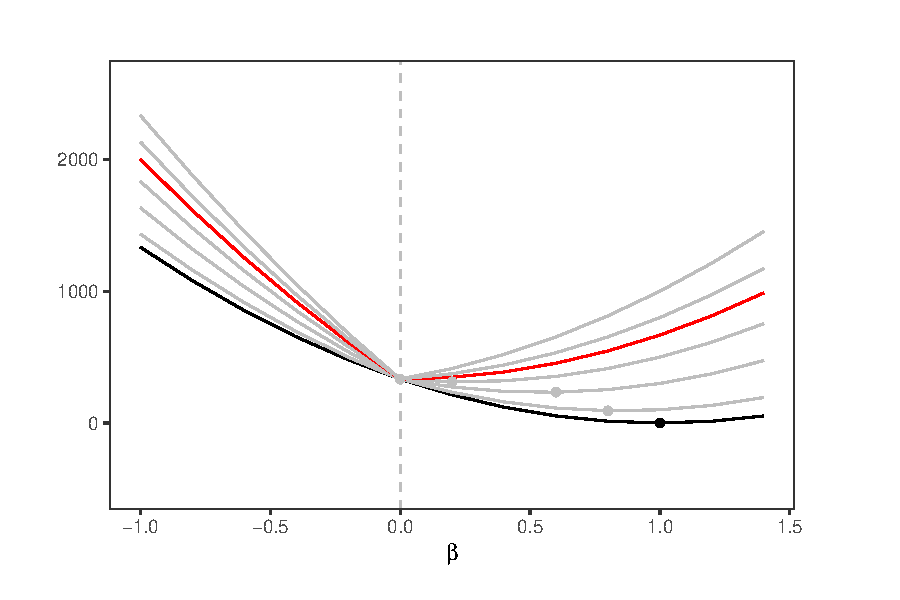
\includegraphics[scale=0.8]{figures/lasso.pdf}
 \end{figure}

 \end{frame}
%----------------------------------------------------------------------%
\begin{frame}[fragile]
\frametitle{Lasso Intuition}

\begin{align}
\frac{dL(\beta)^+}{d\beta} &= -2 \sum y_ix_i+ 2 \beta \sum x_i^2 + \lambda \nonumber \\
& = -2 \sum y_ix_i +\beta + \lambda
\end{align}

\begin{align}
\frac{dL(0)^+}{d\beta} &= -2 \sum y_ix_i + \lambda \nonumber 
\end{align}

then, if 

\begin{align}
   \lambda \geq 2 \sum y_ix_i 
\end{align}

we have $\hat{\beta}_{lasso}=0$

 \end{frame}
%----------------------------------------------------------------------%
\begin{frame}[fragile]
\frametitle{Lasso Intuition}
if  $\lambda < 2 \sum y_ix_i $ we have an interior solution

\begin{align}
  -2 \sum y_ix_i + \hat{\beta}_{lasso} + \lambda =0
\end{align}

\bigskip
\begin{align}
    \hat{\beta}_{lasso} =\sum y_ix_i  - \frac{\lambda}{2}
\end{align}

\bigskip
\begin{align}
    \hat{\beta}_{lasso} =  \hat{\beta}_{OLS} - \frac{\lambda}{2}
\end{align}

\end{frame}

%----------------------------------------------------------------------%
\subsection{Ridge}
%----------------------------------------------------------------------%
\begin{frame}[fragile]
\frametitle{Ridge}

\begin{itemize}
\item For $\lambda \geq 0$ given, consider minimizing the following objective function


\begin{align}
min_{\beta} R(\beta) = \sum_{i=1}^n (y_i-x_i'\beta)^2 + \lambda \sum_{s=2}^p (\beta_s)^2
\end{align}

\bigskip
\item Note:
\begin{itemize}
  \item Intuition is similar to Lasso, however the problem is completely different
\end{itemize}
\end{itemize}


\end{frame}
%----------------------------------------------------------------------%
\begin{frame}[fragile]
\frametitle{Ridge}
\begin{align}
min_{\beta} R(\beta) = \sum_{i=1}^n (y_i-x_i'\beta)^2 + \lambda  (\beta_s)^2
\end{align}

FOC

\begin{align}
-2 \sum_{i=1}^n  y_i x_i + 2\beta + 2 \lambda  \beta_s =0
\end{align}

\begin{align}
\hat{\beta}_{ridge} &= \frac{\sum_{i=1}^n  y_i x_i}{(1+ \lambda)} \nonumber \\
                    &= \frac{\beta_{OLS}}{(1+ \lambda)}
\end{align}

\begin{itemize}
\item Solution is {\it always} interior (unlike Lasso)
\item Solutions is "shrunken"
\end{itemize}
\end{frame}

%----------------------------------------------------------------------%
\begin{frame}[fragile]
\frametitle{Lasso and Ridge Intuition}

   \begin{figure}[H] \centering
            \captionsetup{justification=centering}
              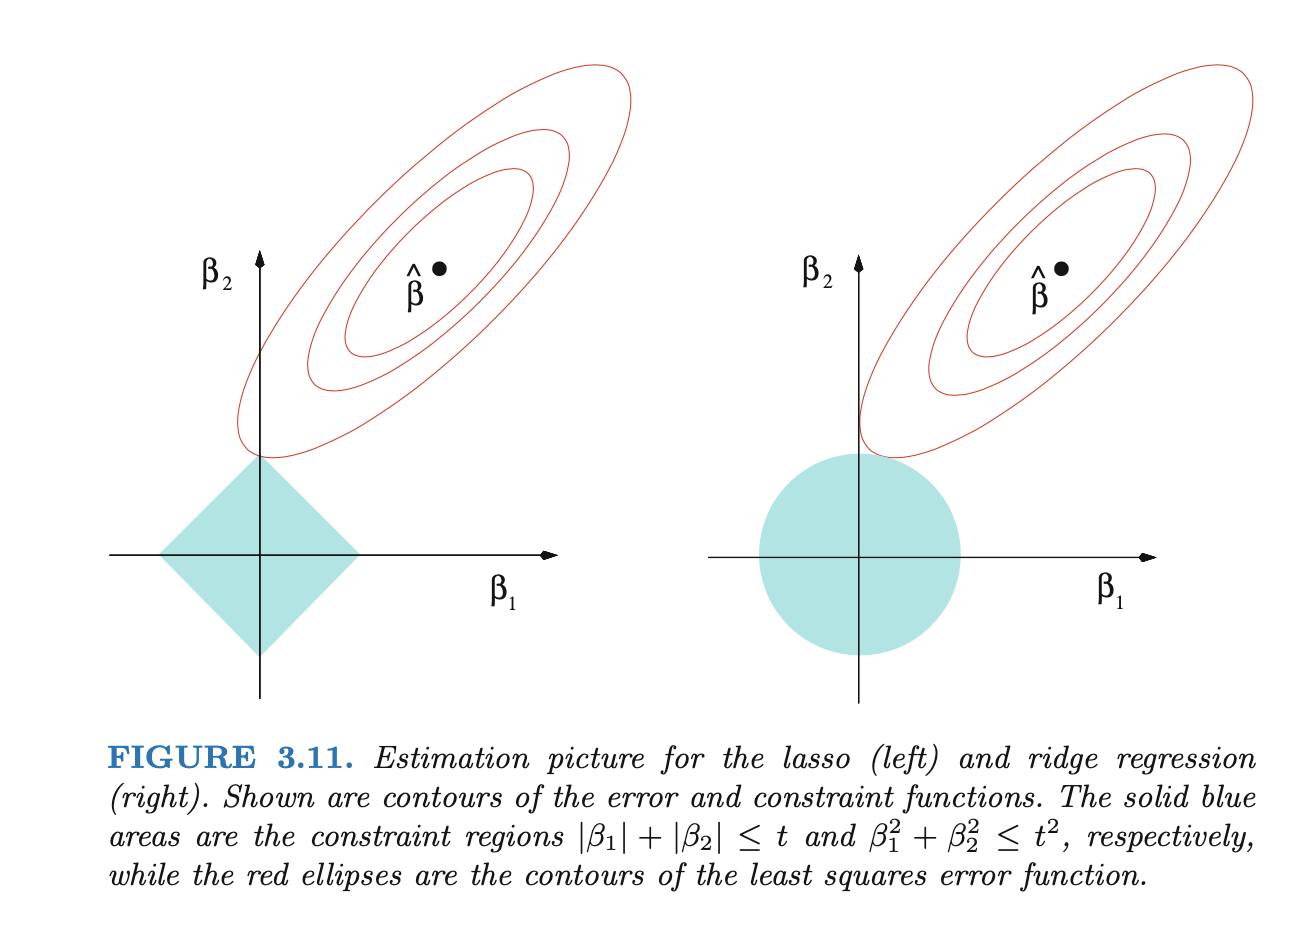
\includegraphics[scale=0.4]{figures/lasso_ridge}
 \end{figure}

 \end{frame}
%----------------------------------------------------------------------%
\begin{frame}[fragile]
\frametitle{Technical comments}

\begin{itemize}
 \item We showed that Ridge is biased, but for certain $\lambda$ $MSE(\beta_{ridge})<MSE(\beta_{OLS})$
 \bigskip
 \item Not possible to derive an exact result for Lasso, but ridge approximates to lasso
 \bigskip
 \item Lasso shrinks everything towards zero, Ridge not quite so
 \bigskip
 \item Application wise:
\begin{itemize}
 \item Standardize the data
 \bigskip
 \item Selection of $\lambda$?
\end{itemize}
\end{itemize}

 \end{frame}
%----------------------------------------------------------------------%
\begin{frame}[fragile]
\frametitle{Technical comments: $\lambda$ Selection}
\begin{itemize}
 \item Selection of $\lambda$?
 \bigskip
 \item Use CV
 \bigskip
 \item Choose a grid of $\lambda$ values, and compute the CV error for each value
 \item Select the $\lambda^*$ that minimizes the prediction error
 \item Estimate using all the observations and the selected $\lambda^*$

\end{itemize}

\end{frame}

%----------------------------------------------------------------------%
\subsection{Extension}
%----------------------------------------------------------------------%
\begin{frame}[fragile]
\frametitle{Extension}

\begin{itemize}
\item Family of penalized regressions

\begin{align}
min_{\beta} R(\beta) = \sum_{i=1}^n (y_i-x_i'\beta)^2 + \lambda \sum_{s=2}^p |\beta_s|^p
\end{align}

 \begin{figure}[H] \centering
            \captionsetup{justification=centering}
              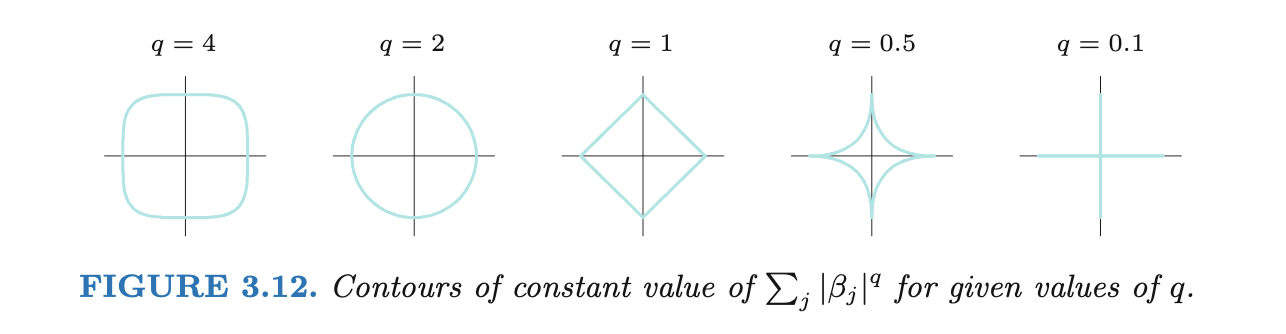
\includegraphics[scale=0.4]{figures/penalties.png}
 \end{figure}
\item  Combination? Elastic Net

\begin{align}
min_{\beta} EL(\beta) &= \sum_{i=1}^n (y_i-x_i'\beta)^2 + \lambda_1 \sum_{s=2}^p |\beta_s| + \lambda_2 \sum_{s=2}^p \beta_s^2 \nonumber \\
 &= \sum_{i=1}^n (y_i-x_i'\beta)^2 + \lambda \sum_{s=2}^p \left(  (1-\alpha) \beta_s^2 + \alpha  |\beta_s|\right)
\end{align}

\end{itemize}
\end{frame}
%----------------------------------------------------------------------%
\subsection{Demo Regularization}
%----------------------------------------------------------------------%
\begin{frame}[fragile]
\frametitle{Demo Regularization}

\begin{tiny}


\begin{Shaded}
\begin{Highlighting}[]
\NormalTok{lambda \textless{}{-}}\StringTok{ }\DecValTok{10}\OperatorTok{\^{}}\KeywordTok{seq}\NormalTok{(}\OperatorTok{{-}}\DecValTok{2}\NormalTok{, }\DecValTok{3}\NormalTok{, }\DataTypeTok{length =} \DecValTok{10}\NormalTok{)}
\NormalTok{lasso \textless{}{-}}\StringTok{ }\KeywordTok{train}\NormalTok{(}
\NormalTok{  price }\OperatorTok{\textasciitilde{}}\NormalTok{., }\DataTypeTok{data =}\NormalTok{ matchdata, }\DataTypeTok{method =} \StringTok{"glmnet"}\NormalTok{,}
  \DataTypeTok{trControl =} \KeywordTok{trainControl}\NormalTok{(}\StringTok{"cv"}\NormalTok{, }\DataTypeTok{number =} \DecValTok{10}\NormalTok{),}
  \DataTypeTok{tuneGrid =} \KeywordTok{expand.grid}\NormalTok{(}\DataTypeTok{alpha =} \DecValTok{1}\NormalTok{, }
  \DataTypeTok{lambda=}\NormalTok{lambda), }\DataTypeTok{preProcess =} \KeywordTok{c}\NormalTok{(}\StringTok{"center"}\NormalTok{, }\StringTok{"scale"}\NormalTok{)}
\NormalTok{  )}
\NormalTok{lasso}
\end{Highlighting}
\end{Shaded}
\end{tiny}
\begin{tiny}

\begin{verbatim}

## 3204 samples
##   17 predictor
## 
## Pre-processing: centered (26), scaled (26) 
## Resampling: Cross-Validated (10 fold) 
## Summary of sample sizes: 2884, 2885, 2882, 2883, 2885, 2883, ... 
## Resampling results across tuning parameters:
## 
##   lambda        RMSE      Rsquared   MAE     
##   1.000000e-02  74410.32  0.7487304  48120.44
##   3.593814e-02  74410.32  0.7487304  48120.44
##   1.291550e-01  74410.32  0.7487304  48120.44
##   4.641589e-01  74410.32  0.7487304  48120.44
##   1.668101e+00  74410.32  0.7487304  48120.44
##   5.994843e+00  74410.32  0.7487304  48120.44
##   2.154435e+01  74410.32  0.7487304  48120.44
##   7.742637e+01  74411.91  0.7487131  48102.41
##   2.782559e+02  74485.72  0.7481557  48011.74
##   1.000000e+03  74702.02  0.7467291  47865.45
## 
## Tuning parameter 'alpha' was held constant at a value of 1
## RMSE was used to select the optimal model using the smallest value.
## The final values used for the model were alpha = 1 and lambda = 21.54435.
\end{verbatim}
\end{tiny}
\end{frame}
%----------------------------------------------------------------------%
\begin{frame}[fragile]
\frametitle{Demo Regularization}

\begin{tiny}
\begin{Shaded}
\begin{Highlighting}[]
\NormalTok{ridge \textless{}{-}}\StringTok{ }\KeywordTok{train}\NormalTok{(}
\NormalTok{  price }\OperatorTok{\textasciitilde{}}\NormalTok{., }\DataTypeTok{data =}\NormalTok{ matchdata, }\DataTypeTok{method =} \StringTok{"glmnet"}\NormalTok{,}
  \DataTypeTok{trControl =} \KeywordTok{trainControl}\NormalTok{(}\StringTok{"cv"}\NormalTok{, }\DataTypeTok{number =} \DecValTok{10}\NormalTok{),}
  \DataTypeTok{tuneGrid =} \KeywordTok{expand.grid}\NormalTok{(}\DataTypeTok{alpha =} \DecValTok{0}\NormalTok{,}\DataTypeTok{lambda=}\NormalTok{lambda), }\DataTypeTok{preProcess =} \KeywordTok{c}\NormalTok{(}\StringTok{"center"}\NormalTok{, }\StringTok{"scale"}\NormalTok{)}
\NormalTok{  )}
\NormalTok{ridge}
\end{Highlighting}
\end{Shaded}
\end{tiny}
\begin{tiny}
\begin{verbatim}
## 3204 samples
##   17 predictor
## 
## Pre-processing: centered (26), scaled (26) 
## Resampling: Cross-Validated (10 fold) 
## Summary of sample sizes: 2884, 2883, 2883, 2884, 2884, 2883, ... 
## Resampling results across tuning parameters:
## 
##   lambda        RMSE      Rsquared   MAE     
##   1.000000e-02  75133.92  0.7479252  47361.73
##   3.593814e-02  75133.92  0.7479252  47361.73
##   1.291550e-01  75133.92  0.7479252  47361.73
##   4.641589e-01  75133.92  0.7479252  47361.73
##   1.668101e+00  75133.92  0.7479252  47361.73
##   5.994843e+00  75133.92  0.7479252  47361.73
##   2.154435e+01  75133.92  0.7479252  47361.73
##   7.742637e+01  75133.92  0.7479252  47361.73
##   2.782559e+02  75133.92  0.7479252  47361.73
##   1.000000e+03  75133.92  0.7479252  47361.73
## 
## Tuning parameter 'alpha' was held constant at a value of 0
## RMSE was used to select the optimal model using the smallest value.
## The final values used for the model were alpha = 0 and lambda = 1000.
\end{verbatim}
\end{tiny}
\end{frame}
%----------------------------------------------------------------------%
\begin{frame}[fragile]
\frametitle{Demo Regularization}

\begin{tiny}
\begin{Shaded}
\begin{Highlighting}[]
\NormalTok{el \textless{}{-}}\StringTok{ }\KeywordTok{train}\NormalTok{(}
\NormalTok{  price }\OperatorTok{\textasciitilde{}}\NormalTok{., }\DataTypeTok{data =}\NormalTok{ matchdata, }\DataTypeTok{method =} \StringTok{"glmnet"}\NormalTok{,}
  \DataTypeTok{trControl =} \KeywordTok{trainControl}\NormalTok{(}\StringTok{"cv"}\NormalTok{, }\DataTypeTok{number =} \DecValTok{10}\NormalTok{), }\DataTypeTok{preProcess =} \KeywordTok{c}\NormalTok{(}\StringTok{"center"}\NormalTok{, }\StringTok{"scale"}\NormalTok{)}
\NormalTok{  )}
\NormalTok{el}
\end{Highlighting}
\end{Shaded}
\end{tiny}
\begin{tiny}

\begin{verbatim}
## glmnet 
## 
## 3204 samples
##   17 predictor
## 
## Pre-processing: centered (26), scaled (26) 
## Resampling: Cross-Validated (10 fold) 
## Summary of sample sizes: 2885, 2885, 2883, 2884, 2883, 2884, ... 
## Resampling results across tuning parameters:
## 
##   alpha  lambda      RMSE      Rsquared   MAE     
##   0.10     230.7569  74163.82  0.7525328  48112.63
##   0.10    2307.5689  74241.34  0.7518849  47772.50
##   0.10   23075.6893  76941.03  0.7489116  48065.77
##   0.55     230.7569  74161.27  0.7524710  48056.67
##   0.55    2307.5689  74420.59  0.7505525  47656.06
##   0.55   23075.6893  82931.37  0.7161268  52413.46
##   1.00     230.7569  74189.84  0.7522040  48029.77
##   1.00    2307.5689  74622.97  0.7493269  47527.50
##   1.00   23075.6893  88016.04  0.6846917  57561.95
## 
## RMSE was used to select the optimal model using the smallest value.
## The final values used for the model were alpha = 0.55 and lambda = 230.7569.
\end{verbatim}
\end{tiny}
\end{frame}
%----------------------------------------------------------------------%
\begin{frame}[fragile]
\frametitle{Demo Regularization}

\begin{scriptsize}
\begin{Shaded}
\begin{Highlighting}[]
\NormalTok{models \textless{}{-}}\StringTok{ }\KeywordTok{list}\NormalTok{(}\DataTypeTok{ridge =}\NormalTok{ ridge, }\DataTypeTok{lasso =}\NormalTok{ lasso, }\DataTypeTok{elastic =}\NormalTok{ el)}
\KeywordTok{resamples}\NormalTok{(models) }\OperatorTok{\%\textgreater{}\%}\StringTok{ }\KeywordTok{summary}\NormalTok{( }\DataTypeTok{metric =} \StringTok{"RMSE"}\NormalTok{)}
\end{Highlighting}
\end{Shaded}
\end{scriptsize}
\begin{tiny}
\begin{verbatim}
## 
## Call:
## summary.resamples(object = ., metric = "RMSE")
## 
## Models: ridge, lasso, elastic 
## Number of resamples: 10 
## 
## RMSE 
##             Min.  1st Qu.   Median     Mean  3rd Qu.     Max. NA's
## ridge   64485.44 70582.29 74874.23 75133.92 77717.74 89880.65    0
## lasso   66245.34 71294.79 74792.57 74410.32 78080.16 80946.67    0
## elastic 59004.20 69395.53 71960.20 74161.27 78485.49 88578.06    0
\end{verbatim}
\end{tiny}

\end{frame}

%----------------------------------------------------------------------%
\begin{frame}[fragile]
\frametitle{Demo Regularization}

   \begin{figure}[H] \centering
            \captionsetup{justification=centering}
              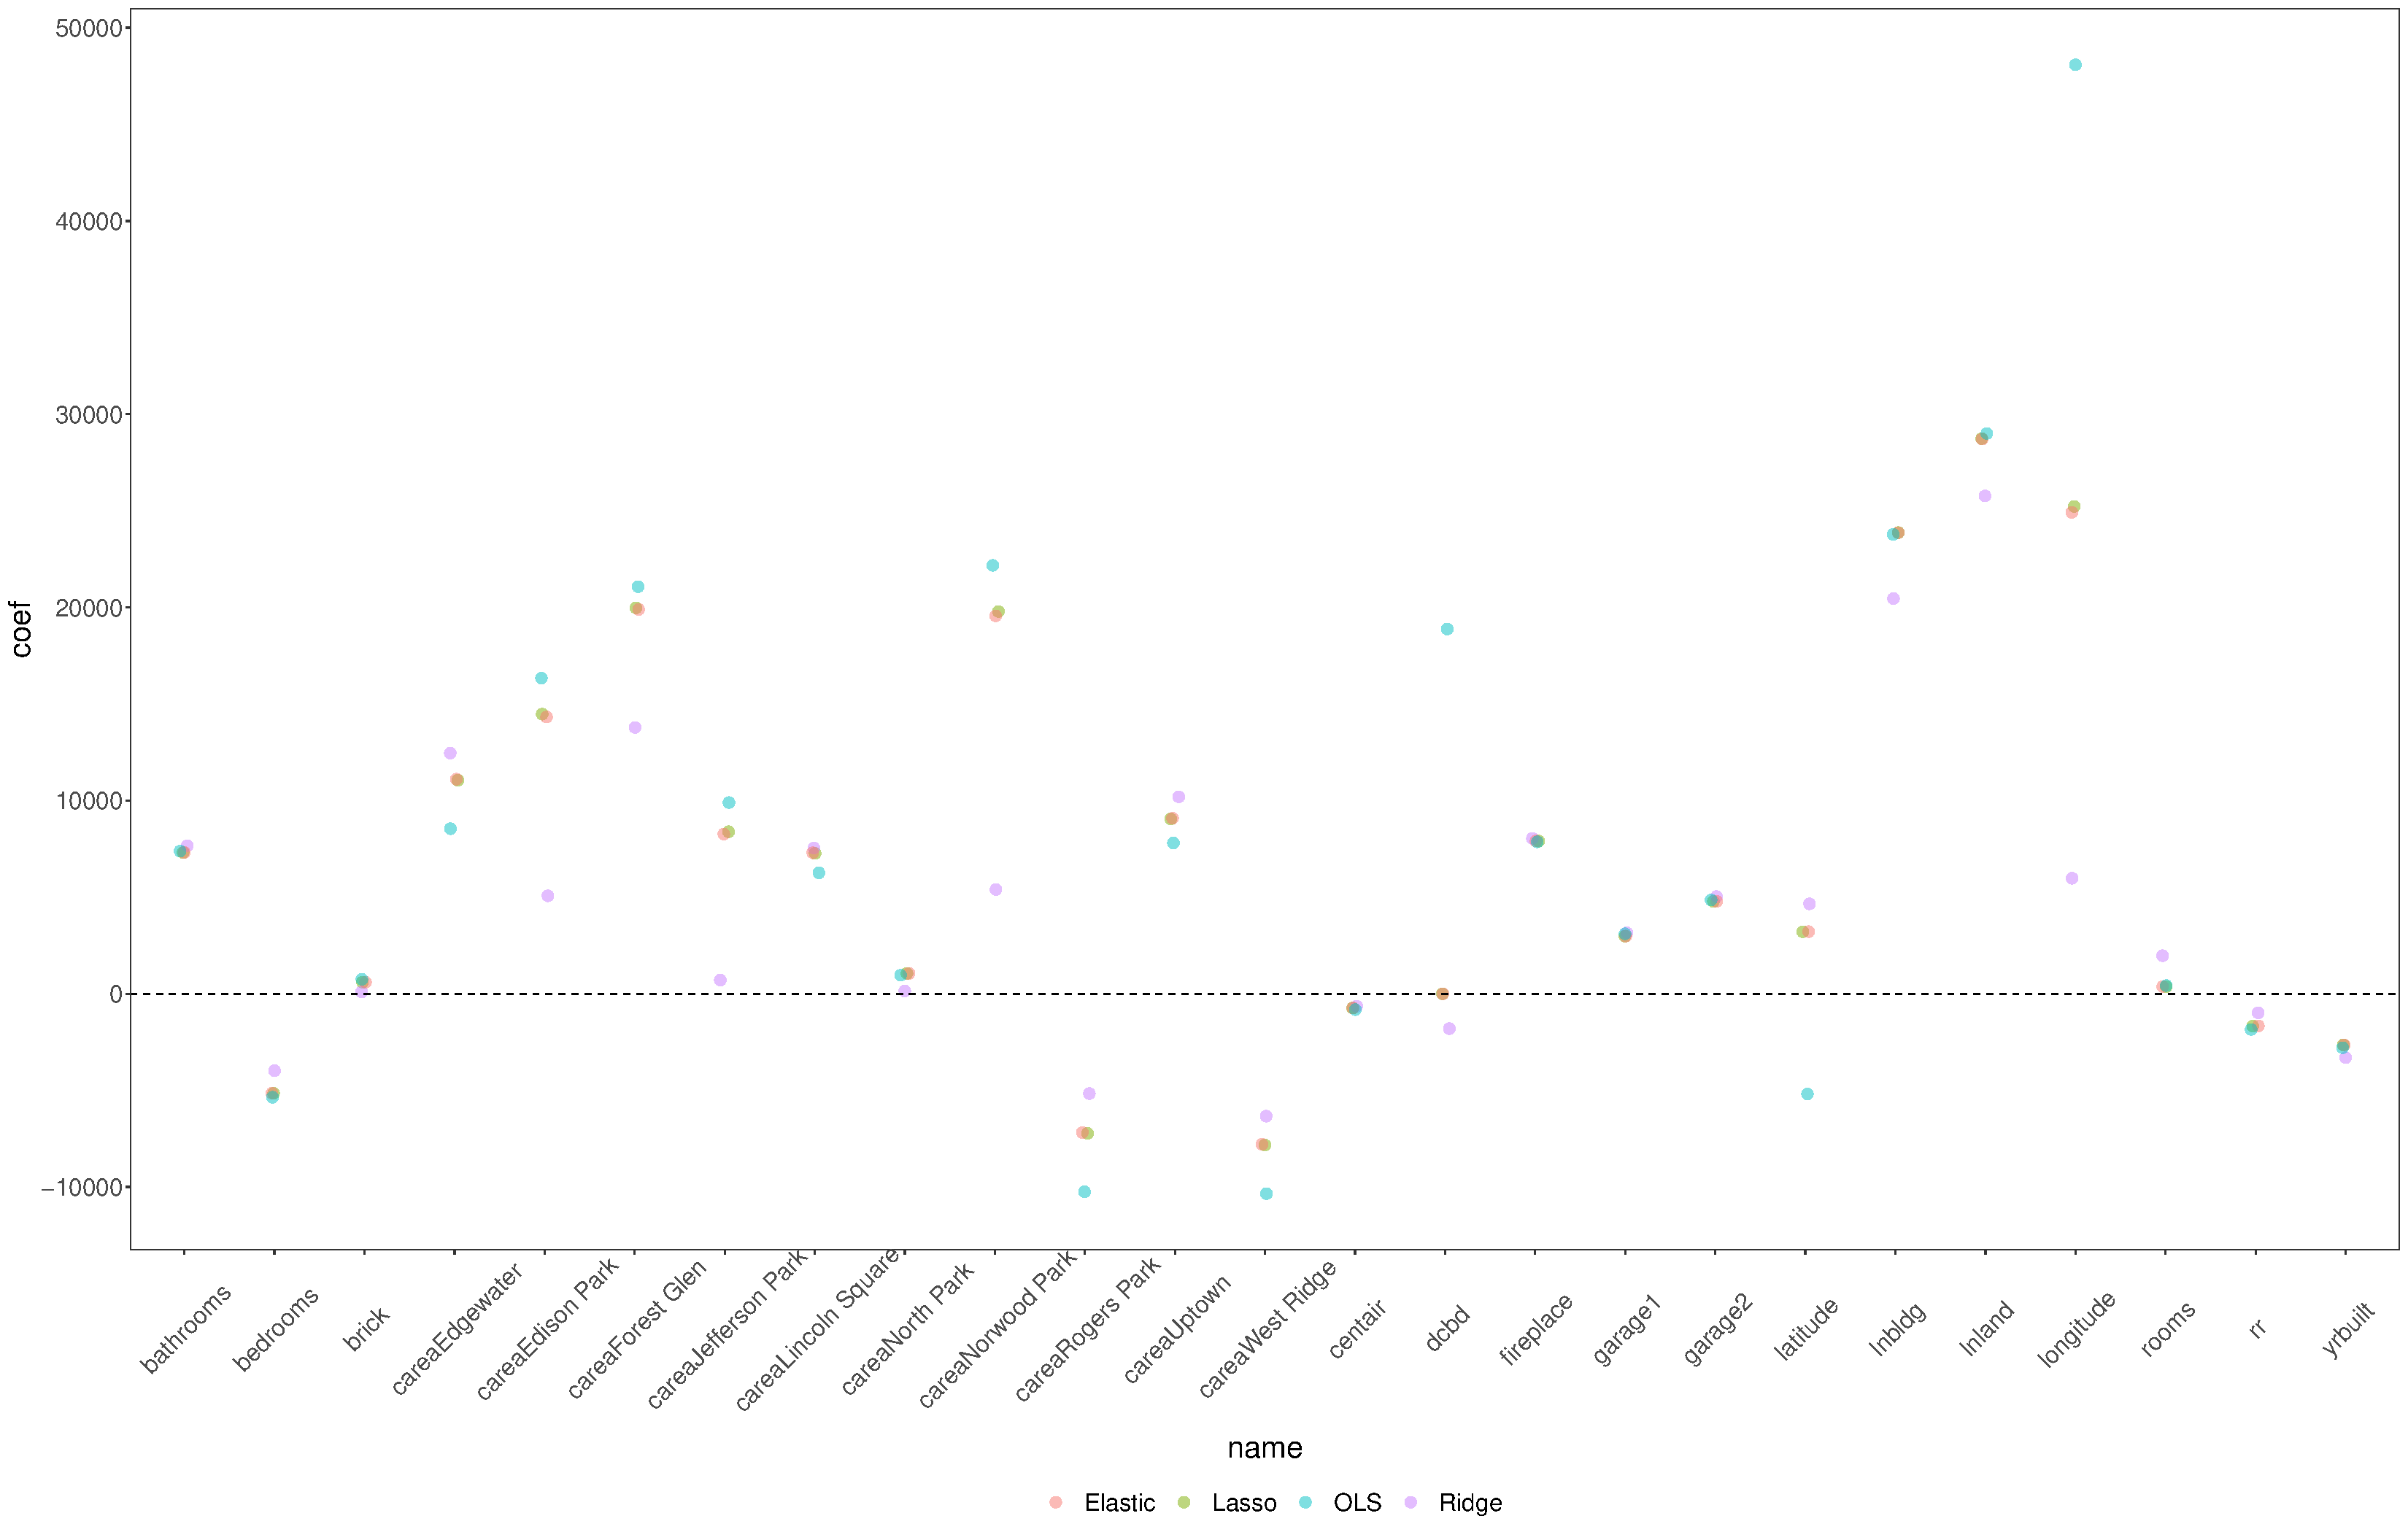
\includegraphics[scale=0.2]{figures/comp}
 \end{figure}

 \end{frame}
%----------------------------------------------------------------------%
\section{Further Readings}
%----------------------------------------------------------------------%
\begin{frame}
\frametitle{Further Readings}

\begin{itemize}


  \item Friedman, J., Hastie, T., \& Tibshirani, R. (2001). The elements of statistical learning (Vol. 1, No. 10). New York: Springer series in statistics.
  \medskip
  \item James, G., Witten, D., Hastie, T., \& Tibshirani, R. (2013). An introduction to statistical learning (Vol. 112, p. 18). New York: springer.
  \medskip
  \item Kuhn, M. (2012). The caret package. R Foundation for Statistical Computing, Vienna, Austria. \url{https://topepo.github.io/caret/index.html}
  \medskip
  \item Taddy, M. (2019). Business data science: Combining machine learning and economics to optimize, automate, and accelerate business decisions. McGraw Hill Professional.

  
\end{itemize}

\end{frame}






%----------------------------------------------------------------------%
%----------------------------------------------------------------------%
\end{document}
%----------------------------------------------------------------------%
%----------------------------------------------------------------------%

